\chapter{Introduction}
\label{introduction}
Music streaming services have an immense amount of power in the music industry. The top streaming services dictate the rules which artists have to play by. The top 5 streaming services form an oligarchy, and the same goes for the top 3 labels. This leads to a centralization of power, and problems related to IT gatekeeping and platformization.

\section{Centralization of power}
Firstly, corporations with power squeeze the music production side by taking large cuts of revenue from the user subscription money. As a result, the artists receive a low compensation. Especially independent artists have a hard time making a living. The distributors Spotify, iTunes and Google Play take on average a 25\% cut for signed records and 40\% cut for unsigned records.

Secondly, Big Tech has curatorial power to decide what is shown in the catalog of their application. The music catalog may seem endless, but in reality it is controlled by the Big Tech corporation and dictated by the interests of major labels. The inner workings of recommendation algorithms and playlists are in the hands of a few labels and streaming services.

Finally, the streaming oligarchy can sensor tracks. The freedom of artist expression is then decided by undemocratic judgments. Big Tech has the power to decide the future of an artist.

\section{Proposed solution: MusicDAO}
This thesis proposes an alternative technology from Big Tech streaming services. We design and implement a decentralized system which attempts to replace the full value chain in music streaming industry, from the subscription money to the artist, by removing all intermediaries and giving power back to the artists and listeners. Listeners can stream music without being dependent on a single provider and can give money directly to artists. Artists receive 100\% of this donation and subscription money.

In essence, the solution is a decentralized autonomous organization (DAO) which is formed by listeners and artists. In this paper we present the design and implementation of our mobile android app MusicDAO. Users of this app form a phone-to-phone serverless network they form a network over which they publish music, download music and transfer money. Peer-to-peer communication and peer-to-peer payments are essential technologies for this. No external servers, third parties or intermediaries are necessary to keep this flow of music and money going. Any person can join the network, publish music and get paid for it. 

MusicDAO supports the following functionalities:
\begin{itemize}
    \item Defining and publishing music content with metadata;
    \item Streaming music over BitTorrent;
    \item Caching and streaming optimization algorithms;
    \item Browsing playlists;
    \item Remote keyword search;
    \item Peer-to-peer donations to artists using Bitcoin.
\end{itemize}

\subsection{Experimentation and evaluation}
In a real-world experiment with Android phones, we tested the feasibility of such a phone-to-phone serverless system. We ran MusicDAO on at least X android devices, and registered the latency of retrieving music metadata, and transaction speeds of transferring money and audio files. 

% Music artists have a hard time making a living. The oligarchical power of music streaming services and labels squeeze  the  production  size  of  the  music  industry
% Stolen from Resonate.is:
% The music industry is dysfunctional. Power has become consolidated in the hands of a small number of technology companies and dominant major labels.
\begin{figure}
	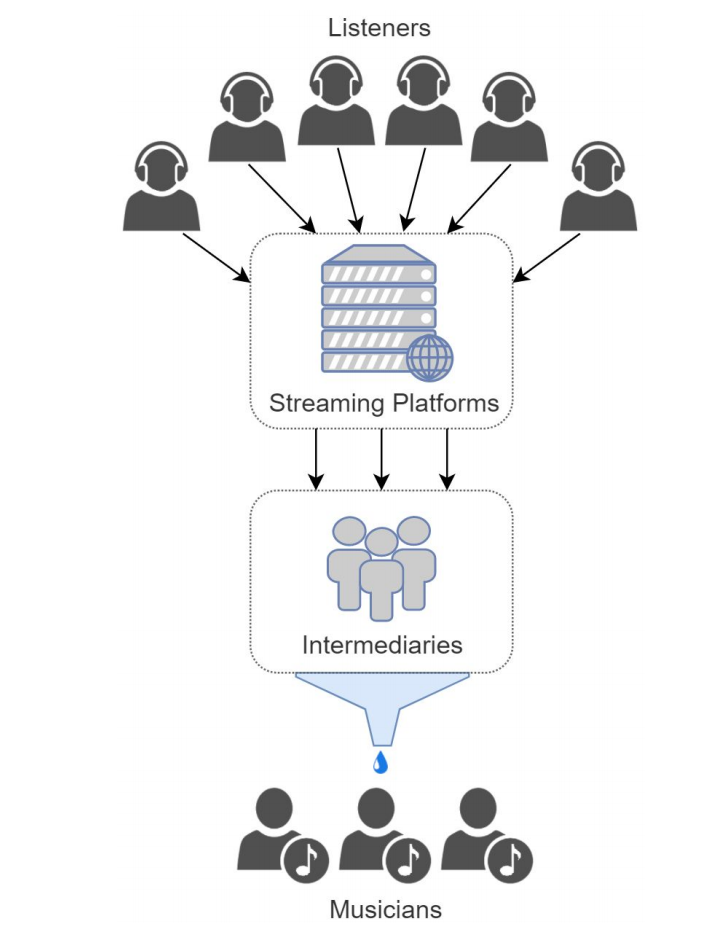
\includegraphics[width=0.3\textwidth]{introduction/problem-image.png}
	\caption{Artist compensation inconsistency}
\end{figure}

% Section X describes the design of the system, section Y its implementation and Z its testing results.
% Most important: How can artists distribute and sell their work in a digital economy beholden to ruthlessly commercial and centralized interests?
% https://thebaffler.com/salvos/the-problem-with-muzak-pelly

% From Audius Whitepapter:
% We see a number of specific challenges faced by creatorsand listeners today:1.  There is little to no transparency around the originsof creator payouts (e.g.  number of plays, location,original gross payment before fees)2.  Incomplete  rights  ownership  data  often  preventscontent  creators  from  getting  paid;  instead,  earn-ings accumulate in digital service providers (DSPs)and rights societies3.  There are layers of middlemen and significant timedelay involved in payments to creators4.  Publishing rights are complicated and opaque, withno incentives for the industry to make rights datapublic and accurate5.  Remixes,  covers,  and  other  derivative  content  arelargely censored due to rights management issues6.  Licensing issues prevent DSPs and content from be-ing accessible worldwide
